%% $Id$

\documentclass[12pt]{article}

\usepackage{a4wide}
\usepackage{graphicx}
\usepackage{color}       
\usepackage{bold-extra} %for bold typewriter fonts, needs [CTAN]/fonts/cm/mf-extra/bold
\usepackage{amsmath}
\usepackage[colorlinks=true,citecolor=blue,linkcolor=blue]{hyperref}

%%%%%%%%%%%%%%%%%%%%%%%%%%%%%%%%%%%%%%%%%%%%%%%%%%%%%
%% Macros for comments
\usepackage{amssymb}
\newcounter{comment}

\newcommand{\comminline}[1]{{%
\refstepcounter{comment}%
\ttfamily\small[$\blacksquare$ \textbf{\underline{Comment}
$\sharp$\thecomment:} #1]}}

\newenvironment{commblock}%
{\refstepcounter{comment}%
\begin{quote}\renewcommand{\baselinestretch}{1}
\ttfamily\small$\blacksquare$ \textbf{\underline{Comment} $\sharp$\thecomment:}}%
{\end{quote}}


\newcommand{\replline}[1]{{
%\refstepcounter{comment}%
\ttfamily\small[$\blacktriangleright$ \textbf{\underline{Reply}
$\sharp$\thecomment:} #1]}}

\newenvironment{replblock}%
{%\refstepcounter{comment}
\begin{quote}\renewcommand{\baselinestretch}{1}
\ttfamily\small$\blacktriangleright$ \textbf{\underline{Reply} $\sharp$\thecomment:}}%
{\end{quote}}


\definecolor{defbox}{gray}{0.85} 

\newcommand{\defboxitem}[3]{ {\ttfamily \bfseries #1[}\emph{#2}{\ttfamily \bfseries ]} & #3 }
\newcommand{\optboxitem}[3]{ {\ttfamily \bfseries #1} & {\ttfamily \bfseries #2 } & #3 }
\newcommand{\mmacomm}[1]{ {\ttfamily \bfseries #1} }

%%%%%%%%%%%%%%%%%%%%%%%%%%%%%%%%%%%%%%%%%%%%%%%%%%%%%

\begin{document}

\title{\texttt{gepard} --- Compton form factors and observables
                            by evolving moments of GEneral PARton 
                            Distributions}
\author{Version: 0.9.4(unreleased)\footnote{For 
informations contact Kre\v{s}imir Kumeri\v{c}ki, \url{kkumer@phy.hr}}}
\date{July 11th 2008}
\maketitle

\begin{abstract}
Fortran package \texttt{gepard} calculates singlet Compton form factor
$\mathcal{H}$ and corresponding Compton cross-sections, beam charge
asymmetry, \ldots,  as well as
DIS form factor $F_2$ by evolving GPDs in conformal moment space 
from an ansatz shape specified at some input scale.  Together
with \texttt{Minuit} minimization subroutine GPD parameters can be fitted to
experimental DVCS and DIS data. For installation instructions
see README file coming with the package.
\end{abstract}

\tableofcontents
\clearpage

\section{Mellin-Barnes representation of relevant observables}

\subsection{DVCS formulas}  

For small $\xi$, DVCS cross section can be approximated by 
\begin{equation}
\frac{d \sigma_{\rm T}}{d t} = \frac{4 \pi \alpha^2 W^2}{(W^2 + \mathcal{Q}^2)
(2 W^2 + \mathcal{Q}^2)^2} | ^{\rm S}\mathcal{H}(\xi, t, \mathcal{Q}^2)|^2 \Bigg|_{\xi
= \frac{\mathcal{Q}^2}{2 W^2 + \mathcal{Q}^2}} \;,
\label{eq:parsigma}
\end{equation}
where singlet Compton form factor $^{\rm S}\mathcal{H}$ in Mellin-Barnes representation is given by
\begin{equation}
{^{\rm S}{\cal H}}(\xi,\Delta^2,{\cal Q}^2)
= \frac{Q_{S}^2}{2i}\int_{c-i \infty}^{c+ i \infty}\!
dj\,\xi^{-j-1} \left[i + \tan \left(\frac{\pi j}{2}\right) \right]
\mbox{\boldmath $C$}_{j}({\cal Q}^2/\mu^2,\alpha_s(\mu)) 
\mbox{\boldmath $H$}_{j} (\xi,\Delta^2,\mu^2) \;.
\label{eq:CFF}
\end{equation}
DVCS Wilson coefficients $\mbox{\boldmath $C$}_{j}({\cal Q}^2/\mu^2,\alpha_s(\mu))$
are given in Eq. (18) of \cite{Kumericki:2006xx}, while moments of
GPD $\mbox{\boldmath $H$}_{j} (\xi,\Delta^2,\mu^2)$ should be specified
by the user in subroutine \texttt{HJ}, as described in Sect. \ref{ssect:ansatz}, or
within Mathematica session, as described in Sect. \ref{sec:mma}.

In practice it is good to use Mellin-Barnes contour of the form displayed
on Fig.~\ref{fig:MellinBarnes}, with point on the contour given
by $j=c+ye^{i\phi}$, with real parameters $c$ and $\phi$.
The usual textbook Mellin-Barnes contour is obtained by
using $\phi = \pi/2$, but, say, $\phi = 3\pi /4$ gives faster
convergence. As long as no poles are crossed value of the
integral should not depend on the value of $c$. One can
try different values of $c$ and $\phi$ to get best numerical
properties. 
For the default GPD ansatz (\texttt{ANSATZ = 'FIT'}), values of  $c$ = 0.5 or 0.25 are
fine, as well as $\phi = 3\pi/4$. However if one uses different GPD ansatz, one should
be aware of the position of the leading poles and choose $c$ accordingly 
\comminline{In the
future version one should implement some sort of automatic choosing of $c$ depending
on the ansatz.}. Also, if
one uses $\overline{MS}$ scheme and \emph{non-diagonal evolution} (\texttt{SCHEME = 'MSBND'}),
one should not make $\phi$ too big or one runs in the danger of hitting poles of
the evolution operator. In this case $\phi$ only slightly larger than (or
equal to $\pi/2$ is the safest choice.

\begin{figure}
\begin{center}
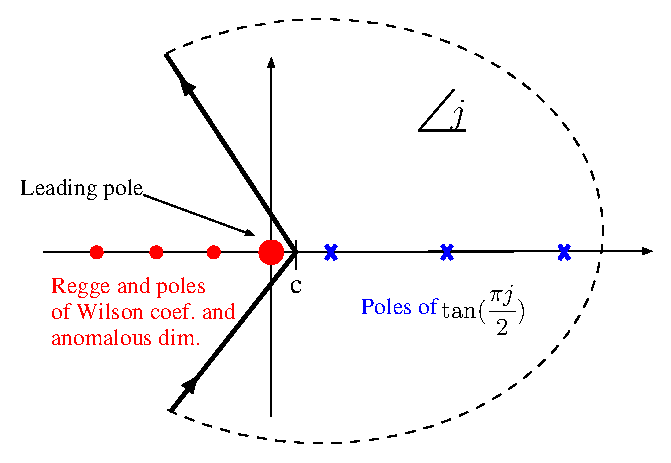
\includegraphics[scale=1.0]{MellinBarnes}
\end{center}
\caption{Contour of the Mellin-Barnes integration.}
\label{fig:MellinBarnes}
\end{figure}


To write the Mellin-Barnes integral in (\ref{eq:CFF}) as an integral
over real variable $y$, one can employ Schwartz reflection principle to
actually integrate over only one of two legs on Fig.~\ref{fig:MellinBarnes}
and write
\begin{multline}
{^{\rm S}{\cal H}}(\xi,\Delta^2,{\cal Q}^2) = Q_{S}^2
\Im\! m\:  e^{i\phi} 
\int_{0}^{\infty} dy \, \xi^{-j-1}
\tan\big(\frac{\pi j}{2}\big)
\mbox{\boldmath $C$}_{j}({\cal Q}^2/\mu^2,\alpha_s(\mu)) 
\mbox{\boldmath $H$}_{j} (\xi,\Delta^2,\mu^2) \\
+ i\: \Im\! m\:  e^{i\phi} 
\int_{0}^{\infty} dy \, \xi^{-j-1}
\mbox{\boldmath $C$}_{j}({\cal Q}^2/\mu^2,\alpha_s(\mu)) 
\mbox{\boldmath $H$}_{j} (\xi,\Delta^2,\mu^2) 
\Bigg|_{j = c + y e^{i\phi}}
\label{<Hformula>}
\end{multline}

\subsection{DIS formulas}  
\label{ssect:DIS}

Similarly, deeply inelastic scattering singlet form-factor ${^{\rm S}\!{F_2}}$ is given by
\begin{eqnarray}
{^{\rm S}\!{F_2}}(\xi,{\cal Q}^2)
&\!\!\!=\!\!\!& \frac{Q_{S}^2}{2 \pi i}\int_{c-i \infty}^{c+ i \infty}\!
dj\,\xi^{-j}
\mbox{\boldmath $C$}^{\rm DIS}_{2,j}(Q^2/\mu^2,\alpha_s(\mu))
\mbox{\boldmath $H$}_{j} (\xi=0,\Delta^2=0,\mu^2) \nonumber \\[2ex]
&\!\!\!=\!\!\!& \frac{Q_{S}^2}{\pi}\, \Im\! m\: e^{i\phi}
\int_{0}^{\infty} dy\:  \xi^{-j}
\mbox{\boldmath $C$}^{\rm DIS}_{2,j}(Q^2/\mu^2,\alpha_s(\mu))
\mbox{\boldmath $H$}_{j} (\xi=0,\Delta^2=0,\mu^2) 
\Bigg|_{j = c + y e^{i\phi}}
\label{<F2formula>}
\end{eqnarray}
DIS Wilson coefficients $\mbox{\boldmath $C$}^{\rm DIS}_{2,j}(Q^2/\mu^2,\alpha_s(\mu))$
are given e.g. in \cite{vanNeerven:2000uj}.

\subsection{Numerical Mellin-Barnes Integration}  
\label{ssect:Integration}
Numerical integration is performed in a way very similar to the one described in
\cite{Vogt:2004ns}: Integrand is largest and
fluctuates most rapidly around zero, mostly due to the factor $\xi^{-j}$. As we
move away from real axis, both
amplitude and oscillation frequency decrease exponentially.
This leads us to divide integration region in exponentially expanding segments
defined by points:
\begin{align*}
0 \,\ldots\, 0.01 & \,\ldots\, 0.025 \,\ldots\, 0.067\,\ldots\, 0.18\,\ldots\, 0.5\,\ldots\, 1.3\,\ldots\, 3.7\,\ldots\, 10. \, \ldots \\
 & \ldots  \, 25. \, \ldots\, 67. \, \ldots\, 182. \, \ldots \, 500. \;,
\label{intervals}
\end{align*}
for \texttt{SPEED=1}, while for higher values of \texttt{SPEED} segments
are defined only using points number $(1, 1+SPEED, 1+ 2 SPEED, \ldots)$ from
the above list (\ref{intervals}).
Here \texttt{SPEED} is one of \texttt{gepard}'s initialization parameters which
controls speed and accuracy of evaluations, see Section \ref{ssect:GEPARD.INI}.
On each segment, standard 8-point Gaussian integration is employed, according
to Eq. (25.4.30) from \cite{AbS65}.
Thus for \texttt{SPEED}=1,2, and 3 we use in total 96, 48, and 32
integration points, respectively. 
One can increase the number of Gaussian points by increasing the parameter
\texttt{ACC} in \texttt{GEPARD.INI}. Number of points on each segment
is $2^{\mbox{\texttt{ACC}}}$,
but default choice is good enough for all practical purposes and increasing this
paremeter serves only as a check of numerical stability.

During the initialization phase, coordinates of points on Mellin-Barnes contour and 
their Gaussian-integration weights
are put on the Fortran common blocks, together with corresponding values of
the moments of Wilson coefficients and anomalous dimensions. 

Also, files with experimental data points, used for fitting, are automatically
inspected, corresponding values of photon virtualities $\mathcal{Q}^2$ are
extracted, and evolution operators for all occuring ratios
$\alpha_{s}(\mathcal{Q}^2)/\alpha_{s}(\mathcal{Q}^{2}_0)$ are also pre-calculated.

Thus these time-demanding evaluations are performed only once.


%\subsection{Ansatz for GPD $\mbox{\boldmath $H$}_{j} (\xi,\Delta^2,\mathcal{Q}_{0}^2)$}
\subsection{Ansatz for GPD}
\label{ssect:ansatz}

User has to provide values of moments of GPDs $\mbox{\boldmath $H$}_{j} 
(\xi,\Delta^2,\mathcal{Q}_{0}^2)$
on an input scale by defining subroutine \texttt{HJ} which has the synopsis
\begin{verbatim}
      SUBROUTINE HJ(J, FCM)
      DOUBLE COMPLEX J, FCM(2)
\end{verbatim}
Input to the subroutine is the complex conformal moment \texttt{J} (i.e. coordinates of a point
on the Melin-Barnes contour), and kinematical parameters \texttt{XI}$=\xi$ and
\texttt{DEL2}$=t=\Delta^2$,
while output should consist of corresponding values
\begin{align}
\texttt{FCM(1)}& =\, ^{\Sigma}\!H_{j} (\xi,\Delta^2,\mathcal{Q}_{0}^2)  \\
\texttt{FCM(2)}& =\, ^{G}\!H_{j}(\xi,\Delta^2,\mathcal{Q}_{0}^2) \,.
\label{eq:FCM}
\end{align}
In the subroutine \texttt{HJ} provided with the software, there are several ansaetze 
already implemented, such as \texttt{ANSATZ='SOFT'} and \texttt{ANSATZ='HARD'}
used in \cite{Kumericki:2006xx}, as well as \texttt{ANSATZ='FITBP'}, used in
\cite{Kumericki:2007sa}.
Twenty four free parameters of this latter ansatz ($N_a$, $\alpha_{a}(0)$, $\alpha_{a}'$,
$M_{0_a}$, $\Delta M_a$ and $p_a$ for  $a = \Sigma, G, u_{\rm val}, d_{\rm val}$),
can either be fixed (e.g. in file \texttt{ansatz.f} used by example programs in
subdirectory \texttt{ex}), or provided by the minimization routine for fitting, see
Fig.~\ref{fig:fit.cmd}.


\section{\texttt{gepard} ingredients}

\begin{itemize}
\item Collection of QCD anomalous dimensions and Wilson coefficients for
unpolarized DIS up to NNLO which can be used for calculating DVCS form factors
in $\overline{CS}$ scheme. For detailed description of (Mathematica) version of
corresponding functions and sources, see the document \texttt{adacf.pdf}.
Collection of QCD anomalous dimensions and Wilson coefficients for singlet DVCS form factors
in $\overline{MS}$ scheme up to NLO.

\item
The evolution of GPDs up to NLO in $\overline{MS}$ scheme 
and  NNLO in $\overline{CS}$ scheme.

\item 
Mellin-Barnes representation for DVCS form-factor ${ }^{\rm S}\mathcal{H}$, and
DIS form-factor ${}^{\rm S}F_2$
\end{itemize}

For calculating and testing DVCS form factors and observables the programs \texttt{test},
\texttt{auxtest}, \texttt{radcorr}, and \texttt{scaledep} are provided at the
moment. For doing example plots many programs are provided in subdirectory \texttt{ex}.

For fitting the GPD parameters using Minuit \cite{James:1975dr}, 
as well as for calculating observables (by
fixing all parameters to desired value), the program \texttt{fit} is provided, and
also Mathematica interface for fitting and evaluating CFF.

\section{Initialization files}
\label{sec:init}

Execution of \texttt{gepard} routines depends on the initialization parameters specified in
the following files
\begin{itemize}
\item  \texttt{GEPARD.INI} --- main initialization for all routines
\item  \texttt{fit.dat} --- which sets of data are used in fits and how are they processed
\item \texttt{fit.cmd} --- Minuit minimization batch file
\item \emph{data files} --- as specified in \texttt{fit.dat}
\end{itemize}
The format and contents of these files should be mostly clear by looking at provided
examples, and detailed explanations follow in the next subsections. Names of the
files used instead of \texttt{fit.dat} and \texttt{fit.cmd} can be specified
as command-line options of fitting program, see Section \ref{sect:examplerun}.

\textbf{NB:} Various constants in these files should be specified
according to Fortran 77 standard! Thus, integers should be without dot (e.g.
\texttt{1}), double precision values with dot and \texttt{'D'} (e.g.
\texttt{1.D0}), while character constants (i.e. strings) should be enclosed in
single quotation marks (e.g. \texttt{'MSBAR'}).

\subsection{\texttt{GEPARD.INI}}
\label{ssect:GEPARD.INI}

File has the structure displayed on Fig.~\ref{fig:GEPARD.INI}.
Only the first column is read by the program and it contains
values of internal Fortran variables specified in the second column and
shortly described in the third one. 
Columns two and three are just convenient reminders for the user. 
Only the first column is read by subroutine \texttt{READPAR} and the
order of entries should correspond to code in that subroutine.  
\begin{figure}[t]
\begin{center}
\hrule
\begin{verbatim}

2          SPEED        1(most accurate), 2 or 3(fastest)
3          ACC          Gaussian subintegrations are on 2**ACC points 
1          P            N^{P}LO order (0, 1 or 2)
4          NF           number of active flavours
1          CZERO        Put to zero to kill LO result
2.5        MU02         scale at which a_strong below is defined
0.0606     ASP(0)       LO  astrong(MU02)/(2 pi)
0.0518     ASP(1)       NLO  astrong(MU02)/(2 pi)
0.0488     ASP(2)       NNLO  astrong(MU02)/(2 pi)
4.0        Q02          GPD input scale
1.0        RF2          ratio {\cal Q}^2/{\mu_{f}^2}
1.0        RR2          ratio {\cal Q}^2/{\mu_{r}^2}
0.5        C            MB integration contour crosses real axis here
1.956      PHI          angle MB contour makes with positive real axis
-0.25      CND          same as C, but for ND evolution MB contour
1.57       PHIND        same as PHI, for ND evolution MB contour
'CSBAR'    SCHEME       'CSBAR', 'MSBAR', 'MSBLO', 'MSBND', 'ZEROG', ...
'FIT'      ANSATZ       GPD ansatz label. Usually FIT, SPLICE or MMA

\end{verbatim}
\hrule
\end{center}
\caption{Example of initialization file \texttt{GEPARD.INI}}
\label{fig:GEPARD.INI}
\end{figure}


\begin{itemize}
\item
\texttt{SPEED} --- \emph{Integer}. Controls the speed and accuracy of the execution. Values can
presently be only 1, 2 and 3, where 1 is the most accurate and at the
same time the slowest case.
As described in Section \ref{ssect:Integration}, \texttt{SPEED} controls the number
of segments in which Mellin-Barnes integration contour is divided before 8-point
Gaussian integration is performed on each segment. It also controls number of
points used for Gaussian integration of partial Compton cross-section over
momentum transfer $t$. This number is 8/\texttt{SPEED}. 

Analysis of how accurate are results for varius \texttt{SPEED} settings can
be found in section \ref{sec:tests}.

\item
\texttt{P} --- \emph{Integer}. Perturbation theory approximation level. 0 = LO, 1 = NLO, and
  2 = NNLO. Because most of the costly evaluations are performed just once,
  during the initialization phase, NLO and NNLO fits take approximately the
  same time, while LO is cca. four times faster. \comminline{This is based
  on just one test, with \texttt{SPEED} = 2.}

\item
\texttt{NF} --- \emph{Integer}. Number of active quark flavors

\item
\texttt{CZERO} --- \emph{Integer}. This multiplies $\alpha_{s}^{0}$ i. e. LO result.
  Should normally be 1, but can be put to 0, so one can get NLO \emph{correction},
  instead of \emph{prediction}, from the routines.

\item
\texttt{MU02} --- \emph{Double precision}. $\mu_{0}^2$ scale at which
$\alpha_s$ input value is specified

\item
\texttt{ASP(0)}, \texttt{ASP(1)}, \texttt{ASP(2)} --- 
\emph{Double precision}. LO, NLO and NNLO $\alpha_{s}(\mu_{0}^2)/(2\pi)$.

\item
\texttt{Q02} --- \emph{Double precision}. Input GPD scale ${\cal Q}_{0}^2$.

\item
\texttt{RF2} --- \emph{Double precision}. $ {\cal Q}^2/{\mu_{f}^2}$ i.e. ratio
of photon virtuality and factorization scale squared.

\item
\texttt{RR2} --- \emph{Double precision}. $ {\cal Q}^2/{\mu_{r}^2}$ i.e. ratio
of photon virtuality and renormalization scale squared.

\item
\texttt{C, PHI} --- \emph{Double precision}. Intercept $c$, and angle $\phi$ of
the Mellin-Barnes contour (Figure \ref{fig:MellinBarnes}).

\item
\texttt{CND, PHIND} --- \emph{Double precision}. Same, but for 
the Mellin-Barnes contour used in the non-diagonal $\overline{MS}$ evolution.

\item
\texttt{SCHEME} --- \emph{Character*5}. Renormalization scheme label. 
Can presently be 
\begin{itemize}
\item \texttt{'CSBAR'}: $\overline{CS}$
\item \texttt{'MSBND'}: $\overline{MS}$, including non-diagonal evolution
\item \texttt{'MSBAR'}: $\overline{MS}$, excluding non-diagonal evolution
\item \texttt{'MSBLO'}: $\overline{MS}$, evolution is LO only
\item \texttt{'ZEROQ'}, \texttt{'TRAJQ'}: $\mbox{\boldmath $C$} = (1,0)$ to all orders
\item \texttt{'ZEROG', \texttt{'TRAJG'}}: $\mbox{\boldmath $C$} = (0,1)$ to all orders
\end{itemize}
Last two are not really renormalization schemes, but just a way to calculate
just a GPD or PDF evolution, without multiplying with Wilson coefficients.
For example, scheme \texttt{'ZEROG'} is used in Sect. \ref{sec:tests} to calculate
evolution of Les Houches benchmark PDFs.

\item
\texttt{ANSATZ} --- \emph{Character*6}. Label of ansatz for conformal moments of GPDs on input scale. 
It should correspond to one of  \texttt{IF\ldots ELSE IF} stanzas in subroutine
\texttt{HJ} in file \texttt{hj.f}. Defaultly implemented ansaetze are
\texttt{TOY} (used in some old development Mathematica notebooks), \texttt{SOFT} and \texttt{HARD},
corresponding to ansaetze from \cite{Kumericki:2006xx}, \texttt{FITBP}, corresponding
to ansatz used in \cite{Kumericki:2007sa}, and \texttt{FIT}, corresponding to a new
ansatz including skewness dependence.

There are also two special values for \texttt{ANSATZ}. First is \texttt{ANSATZ = 'MMA'}, which
can be used if Mathematica interface is active, and
then values for GPDs will be obtained from the ansatz function defined within
Mathematica (see Sect. \ref{sec:mma}). Second is \texttt{ANSATZ = 'SPLICE'}, which
means that GPD is defined in subroutine \texttt{SPLICE} in file \texttt{splice.f}. This
subroutine is automatically created by splicing Fotran code of GPD function originally
defined within Mathematica, but is independent of Mathematica interface (see Sect. \ref{sec:mma}).

\begin{commblock}
This splicing is buggy at the moment and cannot be used!
\end{commblock}

\end{itemize}

Note that \texttt{GEPARD.INI} is meant to be read at the very beginning of the
program execution, and values specified inside can be overridden later. For
example, provided program \texttt{radcorr}, which calculates ratio of NNLO to NLO
radiative corrections, ignores values of \texttt{P}, \texttt{SCHEME} and
\texttt{ANSATZ} in \texttt{GEPARD.INI}, and sets them itself.


\subsection{\texttt{fit.dat}\label{ssect:fitdat}}

\begin{figure}[t]
\begin{center}
\hrule
\begin{verbatim}

'/CPS' 3  2
'START'
'NEWFIG'
'DVCS' '-t' 'dsigma/dt' 0.  1. -1.3  1.2 'BCNST1' 'BCLNST'
'DATA/DVCS_H1_0506_08.DAT'
'DATA/DVCS_H1_0506_09.DAT'
'NEWFIG'
'DVCS' '-t' 'dsigma/dt' 0.  1. -1.3  1.2 'BCNST1' 'BCLNST'
'DATA/DVCS_H1_0506_11.DAT'
'DATA/DVCS_H1_0506_12.DAT'
'CHISQ'
'NEWFIG'
'DVCS' 'Q2' 'sigma' 0.  90. -1.3  1.4 'BCNST1' 'BCLNST'
'DATA/DVCS_H1_3.DAT'
'DATA/DVCS_H1_0506_01.DAT'
'DATA/DVCS_ZEUS_1.DAT'
'CHISQ'
'STOP'
'NEWFIG'
'DIS' 'Q2' 'F2' 0.  50. 0.45  1.5 'BCNST1' 'BCNST'
'DATA/DIS2H1.DAT'
'DATA/DIS4H1.DAT'
'DATA/DIS6H1.DAT'
'CHISQ'

\end{verbatim}
\hrule
\end{center}
\caption{Example of initialization file \texttt{fit.dat}}
\label{fig:fit.dat}
\end{figure}

File has the structure displayed on Fig.~\ref{fig:fit.dat}.


\begin{itemize}

\item 
1$^{\rm st}$ line (\texttt{OUTFORMAT, XPANELS, YPANELS}) ---  \emph{Character*20, Integer, Integer}.
\texttt{OUTFORMAT} specifies which graphical driver should be used according to PGPLOT conventions.
Possible values depend on your installation of PGPLOT. Some useful values are
  \begin{itemize}
  \item \texttt{'/CPS'}  will get output into landscape color Postscript file 
  \item \texttt{'/VCPS'}  will get output into portrait color Postscript file 
  \item \texttt{'/XSERVE'} will get output in an X window (may not work on MS Windows, even
   in cygwin environment)
  \end{itemize}
On one physical page graphs will be arranged on a grid \texttt{XPANELS} 
$\times$ \texttt{YPANELS}.
If PGPLOT is not used, this line is ignored but has to be present and formatted correctly.

\item
Other lines (\texttt{COMMAND}s) --- \emph{Character*20}. Have to be one
of the following things:
\begin{enumerate}
\item 
\texttt{'NEWFIG'} --- New panel of plot is started. All subsequent
datasets, until next \texttt{'NEWFIG'}, will be plotted on the same panel.
In the following row must come a specification of this plot,
in format:
\begin{center}
 \texttt{FIGLABEL, XLABEL, YLABEL, XMIN, XMAX, YMIN, YMAX, XTYPE, YTYPE}
\end{center}
and then PGPLOT will be called as
\begin{verbatim}
CALL PGSWIN (XMIN, XMAX, YMIN, YMAX)
CALL PGBOX (XTYPE, 0.0, 0, YTYPE, 0.0, 0)
CALL PGLAB(XLABEL, YLABEL, FIGLABEL)
\end{verbatim}
see PGPLOT documentation of these functions for details, but apart from
\texttt{XTYPE} and \texttt{YTYPE} purpose of parameters should be obvious.
\item
 Names of files containing the experimental data to be fitted to (see
section \ref{sec:datafiles} for the format of these data files).
\item 
\texttt{'CHISQ'} --- Partial values of $\chi^2$ will be calculated for
  datasets between two \texttt{'CHISQ'} (and between \texttt{'START'} 
and \texttt{'CHISQ'})
\item
\texttt{'START'} or \texttt{'STOP'} --- Only files between \texttt{'START'}
and \texttt{'STOP'} rows will be included in actual fits, while everything beyond
\texttt{'STOP'} is ignored,
\end{enumerate}

\end{itemize}


\subsection{\texttt{fit.cmd}}

\begin{figure}[t]
\begin{center}
\hrule
\begin{verbatim}

0   <--   1=INTERACTIVE   0=BATCH  (Must be 0 on Windows!)
SET TITLE
       Fitting to ansatz: FIT
PARAMETERS
11 'NS        '   0.18      .1  
12 'AL0S      '   1.1       .1   
13 'ALPS      '   0.15      .1  
14 'M02S      '   1.4       .1
15 'DELM2S    '   0.00      .1  
16 'PS        '   3.0       .1  
18 'KAPS      '   1.1       .1  
19 'SKEWS     '   0.9       .1  
21 'NG        '   0.5       .1  
22 'AL0G      '   1.20      .1   
23 'ALPG      '   0.15      .1  
24 'M02G      '   1.1       .1
25 'DELM2G    '   0.00      .1  
26 'PG        '   2.0       .1  
28 'KAPG      '   0.9       .1  
29 'SKEWG     '   1.1       .1  

fix  13 15 16 18 19 23 25 26 28 29
migrad
cali 3

\end{verbatim}
\hrule
\end{center}
\caption{Example of Minuit batch file \texttt{fit.cmd}}
\label{fig:fit.cmd}
\end{figure}

\texttt{fit.cmd} is a file containing Minuit batch commands. Its format is explained in
Minuit manual \cite{Minuit}, Section 3.2.1. The only difference with respect to the
standard Minuit batch file is that first line has to contain integer 1 or 0 as a first
item. This controls whether one will do an interactive Minuit session, or not.
\comminline{At the beginning of the interactive part, one must issue two user-unfriendly
commands, as instructed by the program. This will be made more elegant one day.}
Interactive Minuit session can be very powerful, after one carefully reads Minuit manual.

Second and third line are just giving some label to Minuit session.

Then comes the part where fit parameters are specified.
If one uses default \texttt{ANSATZ = 'FIT'} in
\texttt{GEPARD.INI}, then this part should look like on
Fig.~\ref{fig:fit.cmd}. One could than only change initial values of parameters
(column 3), and maybe their starting step size (column 4).

Last part of this file contains Minuit command instructions. E. g. in the
example on Fig.~\ref{fig:fit.cmd} one first fixes some parameters,
then performs minimization using \texttt{migrad} algorithm,
and finally prints, and maybe plots the results of the fit.

\subsection{Data files\label{sec:datafiles}}

\begin{figure}[t]
\begin{center}
\hrule
\begin{verbatim}

        'SIGMA'                   YOBS
        82.d0                      W
        -1.                        Q2
        6                          N
        3.0   15.7   2.5   3.4   
        5.25   5.7  1.1   1.4  
        8.75  3.20  0.49  0.69
        15.5  1.20  0.22  0.32
        25.0  0.70  0.19  0.19
        55.0  0.15  0.05  0.05


        *     DVCS_H1_3  [H1,  Eur.Phys.J.C44:1-11,2005, hep-ex/0505061] Table 2.
        *       X = Q2,   Y = SIG   (TCUT = - 1 GeV)
        *       W = 82 GeV

\end{verbatim}
\hrule
\end{center}
\caption{Example of an experimental data file \texttt{DVCS\_H1\_3.DAT}.}
\label{fig:DVCS4.DAT}
\end{figure}

Names of these files should be specified in \texttt{fit.dat}, as explained
in Sect. \ref{ssect:fitdat}.
Each data file has the structure displayed on Fig.~\ref{fig:DVCS4.DAT}. In the first
four rows only the first item is read by the program and the second one
(corresponding to internal Fortran variable) is just convenient user
documentation.

\begin{itemize}
\item 
1$^{\rm st}$ row (\texttt{YOBS}) --- \emph{Character*8}. Label of the observable
corresponding to the ``y--axis'' of data. Implemented are labels
  \begin{itemize}
  \item \texttt{'PARSIGMA'} --- Partial Compton cross section $d\sigma/d t$  
  \item \texttt{'SIGMA'} --- Total Compton cross section $\sigma$  
  \item \texttt{'F2'} --- Deeply inelastic scattering form-factor $F_2$  
  \end{itemize} 
(By the way, only first two characters of label strings are significant.)


\item 
2$^{\rm nd}$ row (\texttt{W} or \texttt{X\_BJ}) --- \emph{Double precision}.
In the case of Compton scattering (i.e. \texttt{YOBS} = \texttt{'PARSIGMA'} or
\texttt{YOBS} = \texttt{'SIGMA'}) here is $\gamma^*$ -- proton invariant mass
$W$ (not squared!). In the DIS case (i.e. \texttt{YOBS} = \texttt{'F2'})
here is Bjorken $x$.

\item 
3$^{\rm rd}$ row (\texttt{Q2}) --- \emph{Double precision}. $\mathcal{Q}^2$
for Compton scattering or $Q^2$ for DIS.

Note the following important convention: If one of the quantities that should
be specified in rows 2 or 3 is actually ``x--axis'' of data, this fact
should be specified by putting the \emph{negative number} in the corresponding row!
In other words:
\begin{itemize}
\item 
For \texttt{YOBS} = \texttt{PARSIGMA}, ``x--axis'' variable is 
always $-t = - \Delta^2$, so there are no negative values in second
and third row.
\item 
For \texttt{YOBS} = \texttt{SIGMA}, ``x--axis'' variable is 
either $W$ or $\mathcal{Q}^2$ and corresponding row should have negative number.
\item 
For \texttt{YOBS} = \texttt{F2}, ``x--axis'' variable is 
either Bjorken $x$ or $Q^2$ and corresponding row should have negative number.
\end{itemize}
Thus, the example data on Fig.~\ref{fig:DVCS4.DAT} corresponds to
measurements of total Compton cross section $\sigma(W, \mathcal{Q}^2)$, with
fixed $W = 89\, \textrm{GeV}$, and variable $\mathcal{Q}^2$.

\item 
4$^{\rm th}$ row (\texttt{N}) --- \emph{Integer}. Number of measurements that
follow. Only \texttt{N} next lines will be taken into account, and the
rest of the file is ignored and can be used for comments.

\item
Measurement rows. They consist of four floating point numbers each,
standing for 
\[
 x \qquad y(x) \qquad \Delta y_{\rm stat} \qquad
\Delta y_{\rm syst} \;.
\]
Statistical and systematical errors are combined in quadrature for fitting.

\end{itemize}


\section{An example run}
\label{sect:examplerun}

In the directory where all initialization files named in Section~\ref{sec:init} are
placed one runs executable \texttt{fit}. When minimization is over, and results
printed out (e.g. by Minuit commands \texttt{stop, return, cali 3, \dots}), one 
usually gets three output files:
\begin{itemize}
\item \texttt{fit.mnt}  ---  Output of Minuit routines (When run in batch mode. When
run in the interactive mode one can somehow log the terminal output. For example,
on Linux, by issuing command \texttt{script filename} before the run, and
\texttt{exit} afterwards.)
\item \texttt{OUTFILE.out}   ---  
The file contains the numbers from each processed data file, together with
resulting fit value \texttt{Y(X)\_FIT},
and last column saying how many sigmas is fit value different from experiment.
One stanza from such file is displayed on Fig.~\ref{fig:fitout}.
\item \texttt{OUTFILE.ps}    ---  Almost the same information as 
in \texttt{OUTFILE}.out but in graphical form, as shown on
Fig.~\ref{fig:fitps}  (This works only if you have PGPLOT library. If not, use
executable \texttt{fit\_nopgplot}.). Additionally, \texttt{OUTFILE.ps} has plots
of PDFs and slopes of GPDs using resulting fit parameters.
\end{itemize}

By default \texttt{OUTFILE=fit}, but this can be changed by second command-line
argument of fitting program \texttt{fit}. Thus \texttt{fit  dvcs dvcsnlo test}
will use \texttt{dvcs.dat} instead of \texttt{fit.dat} for reading required
datasets, Minuit commands will be read from \texttt{test.cmd} instead of
\texttt{fit.cmd} and results will go to \texttt{dvcsnlo.out} and \texttt{dvcsnlo.ps} (as well as \texttt{fit.mnt}).



\begin{figure}
\begin{center}
\hrule
\small
\begin{verbatim}

 ------------------------------------------------------------------------
                                    DIS3.DAT                         
      X           Y(X)_FIT      Y(X)_EXP   DY_EXP    (FIT-EXP)/DY_EXP 
 ------------------------------------------------------------------------ 
   0.000200        1.2578        1.2150      0.08         0.5
   0.000320        1.1293        1.0890      0.06         0.7
   0.000500        1.0178        1.0330      0.07        -0.2
   0.000800        0.9110        0.9230      0.05        -0.2
   0.001300        0.8118        0.8110      0.06         0.0
   0.002000        0.7330        0.7700      0.06        -0.6
   0.003200        0.6567        0.5620      0.05         1.8
   0.005000        0.5934        0.6480      0.06        -0.9
   0.008000        0.5359        0.5640      0.06        -0.5 

\end{verbatim}
\hrule
\end{center}
\caption{Example of a part of resulting fit file \texttt{example.out}}
\label{fig:fitout}
\end{figure}

If one has PGPLOT library compiled in, then these fits are as
said before graphed,
in the file \texttt{OUTFILE.ps}. Example graph is shown on Fig.~\ref{fig:fitps}.

\begin{figure}
\begin{center}
\includegraphics[scale=0.72]{examplefit}
\end{center}
\caption{Result of simplified fit to some DVCS and DIS data.}
\label{fig:fitps}
\end{figure}


\section{Tests and accuracy}
\label{sec:tests}

By going to forward limit, as shown in Section~\ref{ssect:DIS}, one can check the accuracy of 
\texttt{gepard} by comparing results with the established DIS routines.
For such comparison we used package {\sc QCD-Pegasus} \cite{Vogt:2004ns} for fast evolution of PDFs.
In particular, we compared evolution of gluonic PDF, which is easiest to compare.

To make \texttt{gepard} calculate only evolution of gluonic PDFs, we use
\texttt{SCHEME} = \texttt{ZEROG} which
makes Wilson coefficient vector equal to $(C_{\Sigma}, C_G) = (0, 1)$
to all orders. Then the same routine that normally calculates DIS form factor
$F_2(x)$ gives $x g(x)$, up
to the charge factor $Q_s$. We also implemented \texttt{ANSATZ} = \texttt{HOUCHE}, corresponding to the
input form of PDFs as used by \cite{Vogt:2004ns}. This is so called Les Houches benchmark PDF
input \cite{Giele:2002hx}.  Finally, to have the same treatment of perturbative expansion of
the solution to RGE, one sets {\sc QCD-Pegasus} parameter \texttt{IMODEV = 3}, as explained in
manual \cite{Vogt:2004ns}. 
Both at NLO and NNLO, we get excellent agreement, with relative differences to
{\sc QCD-Pegasus} results being of the order of $10^{-7}$, as seen on
Fig.~\ref{fig:PDFevol}. \comminline{$x_B \to 1$ limit (not relevant
for small-$x$ calculations) should be improved}


\begin{figure}
\begin{center}
\includegraphics[scale=0.8]{PDFevol}
\end{center}
\caption{Relative difference of NLO (dashed) and NNLO (solid) Les Houches benchmark PDF $x g(x)$
evolved from 2 GeV$^2$ to 10$^4$ GeV$^2$, with respect to referent {\sc QCD-Pegasus} 
\cite{Vogt:2004ns} results.}
\label{fig:PDFevol}
\end{figure}

To see what accuracy can be expected for various values of \texttt{SPEED} parameter 
when calculating total
DVCS cross section, we compare to a referent result obtained using a typical input GPD shape and
maximal \texttt{gepard} precision (\texttt{ACC=6} and \texttt{SPEED=1}, corresponding to
64 points on each integration segment.). Results are shown on
Fig.~\ref{fig:acc}. Here \texttt{ACC = 3} is used, which is the recommended value.
One sees that for  \texttt{SPEED=1} error is always below one per mill, for
\texttt{SPEED=2} it can rise at some values of $\xi$ to a maximum of couple percent, 
but this is usually good
enough. For \texttt{SPEED=3} error is between 15 and 45 percent which may seem
unacceptable for precision analysis, but for fast experimenting with fits it
produces fit results which are often quite similar to those obtained with
smaller \texttt{SPEED} settings.

\begin{figure}
\begin{center}
\includegraphics[scale=0.8]{acc}
\end{center}
\caption{Relative errors of NLO total DVCS cross section when calculated with various
\texttt{SPEED} settings for \texttt{ACC = 3}.}
\label{fig:acc}
\end{figure}



\section{Mathematica interface}
\label{sec:mma}


\subsection{High level functions}

Main ``high level'' functions for accessing Gepard from mathematica are following:

\begin{flushleft}
\colorbox{defbox}{%
\begin{minipage}{\textwidth}%
\begin{tabular}{rp{8cm}}%
\defboxitem{GepardFit}{ \{par1, par2, \ldots\}, options}{Simple fitting of data to 
variable parameters \{par1, par2, \ldots\}} \\[0.8ex]
\defboxitem{JustCali3}{ \{par1, par2, \ldots\}, options}{Just prints out initial chi-square without
any fitting. Useful for checking ansaetze and debugging}\\[0.8ex]
\defboxitem{cffH}{xi, t, q2, q02, options}{Returns singlet Compton form factor
$\mathcal{H}(xi=\xi, t=\Delta^2, q2=\mathcal{Q}^2, q02=\mathcal{Q}_{0}^2)$.}\\[0.8ex]
\defboxitem{cffE}{xi, t, q2, q02, options}{Returns singlet Compton form factor
$\mathcal{E}(xi=\xi, t=\Delta^2, q2=\mathcal{Q}^2, q02=\mathcal{Q}_{0}^2)$.}\\[0.8ex] 
\defboxitem{F2}{xbj, q2, q02, options}{Returns DIS singlet form factor
$F_{2}(xbj=x_{BJ}, q2=\mathcal{Q}^2, q02=\mathcal{Q}_{0}^2)$.}\\[0.8ex] 
\defboxitem{gpdHzero}{x, t, q2, q02, options}{Returns singlet GPD
$H(x, \eta=0, t, q2=\mathcal{Q}^2, q02=\mathcal{Q}_{0}^2)$.}\\[0.8ex] 
\defboxitem{gpdHtraj}{x, t, q2, q02, options}{Returns singlet GPD
$H(x, \eta=x, t, q2=\mathcal{Q}^2, q02=\mathcal{Q}_{0}^2)$.}
\end{tabular}%
\end{minipage}}\\[0.5ex]
{\small High level functions available in \emph{Mathematica} interface.}
\end{flushleft}

Parameters controlling detailed behavior of these functions are specified in
the usual \texttt{GEPARD.INI} file, but important subset of these parameters can
be overriden by \emph{options}:

\begin{flushleft}
\colorbox{defbox}{%
\begin{minipage}{\textwidth}%
\begin{tabular}{llp{8cm}}%
\emph{option name} & \emph{default value} & \\ \hline
\optboxitem{SPEED}{in \emph{GEPARD.INI}}{speed of execution} \\
\optboxitem{P}{in \emph{GEPARD.INI}}{order of perturbation series N$^{P}$LO}\\
\optboxitem{SCHEME}{in \emph{GEPARD.INI}}{factorization scheme (CSBAR, MSBND, \ldots)}\\
\optboxitem{ANSATZ}{in \emph{GEPARD.INI}}{ansatz used (MMA, SPLICE, FIT, \ldots)}\\
\optboxitem{DATFILE}{\emph{fit}}{file DATFILE.dat specifies fitting datasets.}\\
\optboxitem{OUTFILE}{\emph{fit}}{output to go to OUTFILE.out and OUTFILE.ps}
\end{tabular}%
\end{minipage}}\\[0.5ex]
{\small Options of \mmacomm{GepardFit}, \mmacomm{JustCali3}, \mmacomm{cffH}, 
and \mmacomm{cffE}.}
\end{flushleft}

All of these functions expect that user has provided ansatz for GPDs and PDFs
in one of the three following ways, denoted by the corresponding setting
of parameter 'ANSATZ' and ordered by decreasing flexibility and increasing speed:

\begin{description}
\item[\texttt{MMA}] 
Moments of GPDs and PDFs have to be defined as a Mathematica two-element vector function
\mmacomm{GPDMom[j\_,t\_,xi\_]} = \{\mmacomm{GPDMomQ}, \mmacomm{GPDMomG} \}  where 
\mmacomm{GPDMomQ} and \mmacomm{GPDMomG} are expressions for (singlet) quark and gluon GPDs
depending, apart from explicit arguments $j$, $t$, and $xi$, only on
parameters \mmacomm{PAR[n]}, where $n$ corresponds to the elements of first column of the \mmacomm{Parameters}
array described below. (Same for PDFs with \mmacomm{GPD}$\to$\mmacomm{PDF} above.) 
After defining this function, it has to be compiled by issuing command \mmacomm{CompileMoments[]}.

\item[\texttt{SPLICE}] 
One defines moments in exactly the same way as in point 1 above, but then, instead of compiling
them, one transforms them into Fortran form, and puts them into Fortran subroutine
\texttt{SPLICE}. This is automatized by function \mmacomm{SpliceToFortran}. Resulting code
is 10 times faster, but one is limited to ansaetze which can be expressed in terms of available
Fortran functions (log-exp, trigonometric, hyperbolic), or one needs to write some
Fortran code defining required additional functions. Also, after issuing \mmacomm{SpliceToFortran}
one musts recompile Gepard (which usually means just issuing command '\emph{make gepard.exe}')
and reload gepard.exe (which usually means just reevaluating $\langle\langle<<$~\emph{gepard.m}).
\comminline{This \texttt{SPLICE} is somewhat broken at the moment.}

\item[\texttt{FIT}] 
One writes explicitly Fortran code in subroutine 'HJ', following examples there. This
is usually not much faster than 'SPLICE', but can be used to put at ones disposal
many different ansaetze at the same time, by just using additional names.
(At the moment, name 'FIT' denotes the same ansatz as defined in example notebook fit.nb,
name 'FITBP' denotes ansatz used in \cite{Kumericki:2007sa}, 'HARD' and 
'SOFT' denote ansaetze used in \cite{Kumericki:2006xx} etc.)
\end{description}

Apart from speed, one advantage of ansaetze 'SPLICE' and 'FIT' is that they are
available to pure Fortran fitting without the need for Mathematica software.

\begin{flushleft}
\colorbox{defbox}{%
\begin{minipage}{\textwidth}%
\begin{tabular}{rp{8cm}}%
\defboxitem{CompileMoments}{}{Creates ANSATZ 'MMA' with compiled Mathematica 
functions \mmacomm{GPD} and \mmacomm{PDF} called by Fortran via MathLink.} \\[0.8ex]
\defboxitem{SpliceToFortran}{path, substitutions}{Creates ANSATZ `SPLICE' by
creating  Fortran subroutine `SPLICE` with Fortran expressions for ansatz.
\emph{path} is path to gepard/src directory, and 
\emph{substitutions} is a list of replacement rules which should take care of some 
differences in names of Mathematica and Fortran variables and functions.} 
\end{tabular}%
\end{minipage}}\\[0.5ex]
{\small Functions creating ansaetze from Mathematica expressions.}
\end{flushleft}

\subsection{Parameters}

Additionally to ansatz, user has to specify parameters on which ansatz depends and
which will be varied during the fitting process. These parameters must be collected
in the 2D matrix \mmacomm{Parameters} where each row has six entires defining one 
parameter in the form expected by Minuit:

\vspace*{2ex}

\begin{tabular}[h]{|c|c|c|c|c|c|}
\hline
\emph{ID} & \emph{name} & \emph{starting value} & \emph{step} & \emph{lower bound} & 
\emph{upper bound} \\
\hline
\end{tabular}

\vspace*{2ex}

'ID' must be integer, 'name' string of maximally 10 characters, and other are real numbers.
Lower and upper bounds should preferably be 0.0, which means that parameter is unbounded.
See Minuit manual for details.

\subsection{Low level functions}

High level functions are just a canned sequences of low level functions which can
be used for finer control over the whole process. Here is just a list with
descriptions. For details, see example notebook 'fit.nb'.


\begin{flushleft}
\colorbox{defbox}{%
\begin{minipage}{\textwidth}%
\begin{tabular}{rp{8cm}}%
\defboxitem{GepardInit}{options}{Initializes Gepard parameters by first reading GEPARD.INI
and then taking into account \emph{options} which are the same as for 
\mmacomm{GepardFit}. } \\[0.8ex]
\defboxitem{MinuitInit}{integer}{Initializes Minuit, initializes COMMON blocks with evolved
Wilson coefficients and returns coordinates on Mellin-Barnes contour. \emph{integer} is
presently ignored.} \\[0.8ex]
\multicolumn{2}{l}{\mmacomm{MinuitSetParameter[}\emph{id, pname, vstart, step, lo, hi}
\mmacomm{]} } \\
 & Declares Minuit parameter by forwarding arguments to subroutine MNPARM \\[0.8ex]
\defboxitem{MinuitCommand}{string}{sends to Minuit the command \emph{string} by
forwarding it to subroutine MNCOMD. } \\[0.8ex]
\defboxitem{PrintMinuitCommand}{string, fontsize}{same, but prints the Minuit output
by reading \texttt{fit.mnt} file. Useful for Minuit commands such as
``show correlations'' or ``scan''.} \\
\defboxitem{SaveParameters}{}{writes present values of fitting
parameters into the list \texttt{Parameters}, preparing it thus for next fitting procedure or
for evaluation of \texttt{cffH}, \texttt{cffE} or \texttt{F2}.}
\end{tabular}%
\end{minipage}}\\[0.5ex]
{\small Functions controlling fitting procedure. First three should probably not be
used directly at all, but only via calling high level functions. Last two essentially
enable complete Minuit interface from within Mathematica session.}
\end{flushleft}


\begin{flushleft}
\colorbox{defbox}{%
\begin{minipage}{\textwidth}%
\begin{tabular}{rp{8cm}}%
\defboxitem{PrettyStatus}{}{Prints out current fitting result (chi-square, values of
arameters,\ldots) in a nicely formatted form.} \\[0.8ex]
\defboxitem{MinuitStatus}{}{Returns current status of minimization in form of a 
list {chi-square, quality of covariance matrix: 0-3}} \\[0.8ex]
\defboxitem{MinuitGetParameter}{ID}{Returns the current value of a parameter
number \emph{ID} by calling Minuit subroutine MNPOUT. It returns list 
\{\emph{value}, \emph{error estimate}, \emph{internal parameter number} (or \emph{zero} if
constant/fixed, or negative if undefined)\}. } \\[0.8ex]
%\defboxitem{ParameterID}{symbol}{Returns parameter number (ID) of a parameter
%with name \emph{symbol} (not string!), as specified by array Parameters.} \\[0.8ex]
\end{tabular}%
\end{minipage}}\\[0.5ex]
{\small Functions for displaying results I.}
\end{flushleft}


\begin{flushleft}
\colorbox{defbox}{%
\begin{minipage}{\textwidth}%
\begin{tabular}{rp{8cm}}%
\multicolumn{2}{l}{\mmacomm{PlotMinuitContour[}\emph{par1, par2, npts, options}
\mmacomm{]} } \\
 & Plots correlation contour
of parameters par1 and par2 using Minuit's MNCONT \\[0.8ex]
\multicolumn{2}{l}{\mmacomm{PlotMinuitContourFixed[}\emph{par1, par2, npts, options}
\mmacomm{]} } \\
& same, but chi-square
is not minimized with respect to other parameters for each point. Thus
significantly faster. \\[0.8ex]
\multicolumn{2}{l}{\mmacomm{PlotMinuitContourFixedAll[}\emph{par1, par2, npts, options}
\mmacomm{]} } \\
& same, but
also values of par1 and par2 are not changed even if better minimum is found. \\[0.8ex]
\defboxitem{GPD}{flavor, x, t, xi}{Gives value of x-space GPDs (flavor: 1=Q, 2=G). 
It relies on moments \mmacomm{GPDcurrent[j,t,xi]} which are set up automatically
by calling \mmacomm{GepardFit}, \mmacomm{JustCali3} or \mmacomm{PrettyStatus}, and can
be set up manually using ansatz and parameter values. Not to be confused with
\mmacomm{GPD[\{val1, val2, ...\}, t, xi]} which provides ansatz. (Should use
different names in the future.)} \\[0.8ex]
\defboxitem{plotPDFs}{}{Plots GPD[flavor, x, 0, 0] for flavor 1=Q (blue) 
or 2=G (red).} \\[0.8ex]
\defboxitem{slope}{flavor, x}{GPD slope at x} \\[0.8ex]
\defboxitem{plotslopes}{}{Plots GPD slope as a function of x for flavor 1=Q (blue) and
 2=G (red). Slow, better just look at PS file.} \\[0.8ex]
\defboxitem{ChiSquareProbability}{dof, chisq}{Gives probability that chi-square
for a system with \emph{dof} degrees of freedom will be larger than or equal to \emph{chisq}.}
\end{tabular}%
\end{minipage}}\\[0.5ex]
{\small Functions for displaying results II.}
\end{flushleft}

\section{Algorithmic structure of \texttt{gepard} and its subroutines}

Calling graph of subroutines for executable \texttt{fit} is displayed on
Fig.~\ref{fig:callgraph}. Each subroutine,
function and main program is described in the extended \texttt{gepard-api.pdf} documentation,
as well as in hyperlinked HTML documentation 
(\texttt{doc/html/masterindex.html}) produced by 
\texttt{robodoc} automatic documentation generator.

\begin{figure}[ht]
\begin{center}
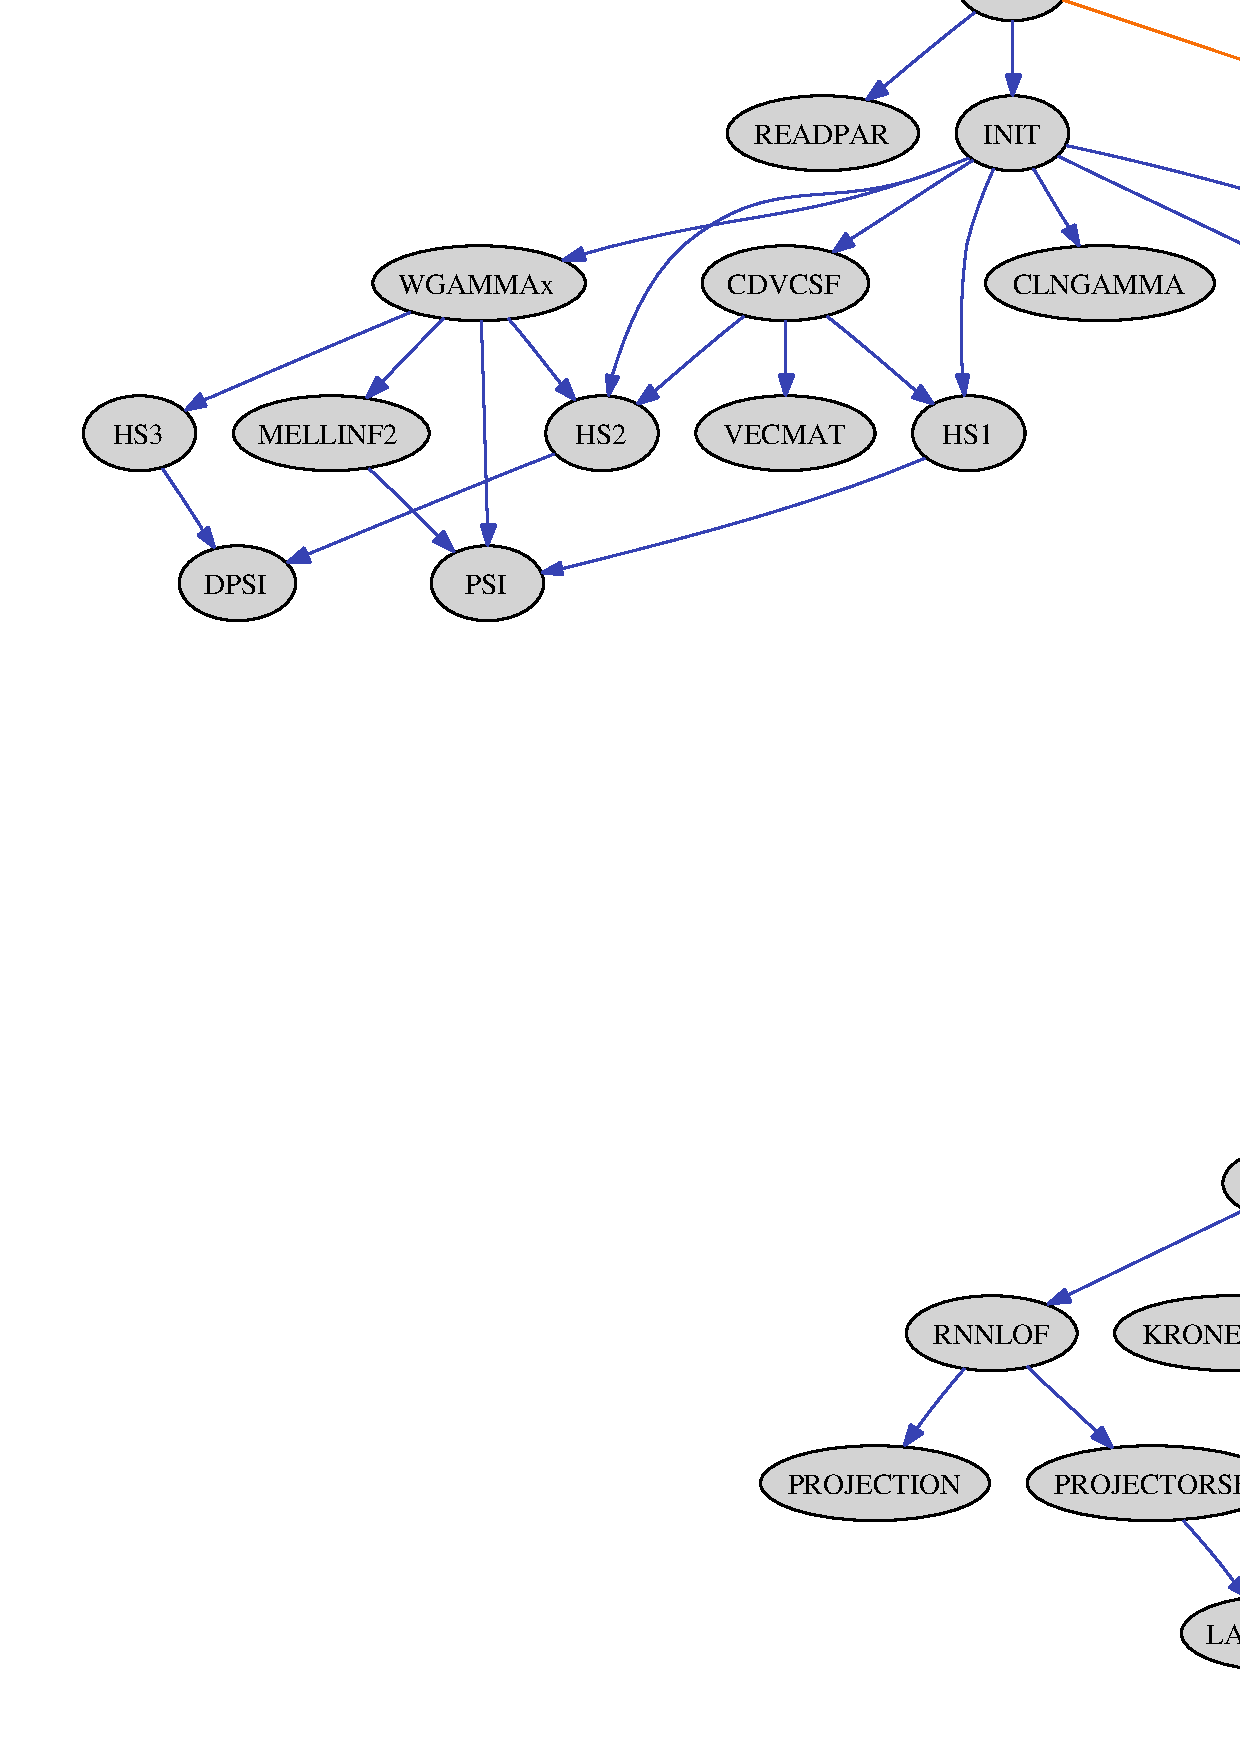
\includegraphics[scale=0.52]{callgraph}
\end{center}
\caption{Calling graph (for slightly older version gepard 0.9.1)}
\label{fig:callgraph}
\end{figure}




%\bibliographystyle{h-physrev4}
\bibliographystyle{JHEP-2}
%\bibliographystyle{mynatbib}
\bibliography{/home/kkumer/Lit/kkumer}



\end{document}

